%% LLT: Turn off some annoying warnings...
\RequirePackage{silence}
\WarningFilter{titlesec}{Non standard sectioning command}
\WarningFilter{scrreprt}{Usage of package}
\WarningFilter{scrreprt}{Activating an ugly workaround}

% **************************************************
% Document Class Definition
% **************************************************
\documentclass[%
	paper=A4,					% paper size --> A4 is default in Germany
%	twoside=true,				% onesite or twoside printing
    oneside=true,
	twoside=false,				% onesite or twoside printing
	openright,					% doublepage cleaning ends up right side
	parskip=full,				% spacing value / method for paragraphs
	chapterprefix=true,			% prefix for chapter marks
	11pt,						% font size
	headings=normal,			% size of headings
	listof=totoc,				% include listof entries in toc
	titlepage=on,				% own page for each title page
	captions=tableabove,		% display table captions above the float env
	draft=false,				% value for draft version
]{scrreprt}%

\usepackage{ngerman}
\usepackage{hyperref}
\usepackage{wrapfig}
\usepackage[export]{adjustbox}
\usepackage{mathtools}
\usepackage{tocloft}
\usepackage{acronym}
\usepackage[utf8]{inputenc}		% defines file's character encoding
\usepackage{paralist}          % for compactitem itemization
\usepackage{chngcntr}           % Einfache Nummerierung von Abbildungen
\usepackage{blindtext}
\counterwithout{figure}{chapter} % Einfache Nummerierung von Abbildungen
\usepackage{listings} % Code Listings

%=====
\lstset{
	language=Python,
	basicstyle=\ttfamily,
	otherkeywords={self},             
	keywordstyle=\ttfamily\color{blue!90!black},
	keywords=[2]{True,False},
	keywords=[3]{ttk},
	keywordstyle={[2]\ttfamily\color{yellow!80!orange}},
	keywordstyle={[3]\ttfamily\color{red!80!orange}},
	emph={def, return},          
	emphstyle=\ttfamily\color{red!80!black},    
	stringstyle=\color{blue!80!black},
	showstringspaces=false            
}
%======
\usepackage{float} % exaktes Figure Placement mit H
\lstset{
  breaklines=true,
%  numbers=left,
  numbersep=5pt,
  basicstyle=\footnotesize\ttfamily,
 % numberstyle=\tiny\color{black}
%  literate=%
%  {Ö}{{\"O}}1
%  {Ä}{{\"A}}1
%  {Ü}{{\"U}}1
%  {ß}{{\ss}}2
%  {ü}{{\"u}}1
%  {ä}{{\"a}}1
%  {ö}{{\"o}}1
}

\lstset{literate=
  {á}{{\'a}}1 {é}{{\'e}}1 {í}{{\'i}}1 {ó}{{\'o}}1 {ú}{{\'u}}1
  {Á}{{\'A}}1 {É}{{\'E}}1 {Í}{{\'I}}1 {Ó}{{\'O}}1 {Ú}{{\'U}}1
  {à}{{\`a}}1 {è}{{\`e}}1 {ì}{{\`i}}1 {ò}{{\`o}}1 {ù}{{\`u}}1
  {À}{{\`A}}1 {È}{{\'E}}1 {Ì}{{\`I}}1 {Ò}{{\`O}}1 {Ù}{{\`U}}1
  {ä}{{\"a}}1 {ë}{{\"e}}1 {ï}{{\"i}}1 {ö}{{\"o}}1 {ü}{{\"u}}1
  {Ä}{{\"A}}1 {Ë}{{\"E}}1 {Ï}{{\"I}}1 {Ö}{{\"O}}1 {Ü}{{\"U}}1
  {â}{{\^a}}1 {ê}{{\^e}}1 {î}{{\^i}}1 {ô}{{\^o}}1 {û}{{\^u}}1
  {Â}{{\^A}}1 {Ê}{{\^E}}1 {Î}{{\^I}}1 {Ô}{{\^O}}1 {Û}{{\^U}}1
  {œ}{{\oe}}1 {Œ}{{\OE}}1 {æ}{{\ae}}1 {Æ}{{\AE}}1 {ß}{{\ss}}1
  {ű}{{\H{u}}}1 {Ű}{{\H{U}}}1 {ő}{{\H{o}}}1 {Ő}{{\H{O}}}1
  {ç}{{\c c}}1 {Ç}{{\c C}}1 {ø}{{\o}}1 {å}{{\r a}}1 {Å}{{\r A}}1
  {€}{{\EUR}}1 {£}{{\pounds}}1
}
\usepackage{color}
\definecolor{javared}{rgb}{0.6,0,0} % for strings
\definecolor{javagreen}{rgb}{0.25,0.5,0.35} % comments
\definecolor{javapurple}{rgb}{0.5,0,0.35} % keywords
\definecolor{javadocblue}{rgb}{0.25,0.35,0.75} % javadoc

% **************************************************
% Debug LaTeX Information
% **************************************************
%\listfiles

% **************************************************
% Information and Commands for Reuse
% **************************************************

\newcommand{\thesisTitle}{\Huge MASTER THESIS}
\newcommand{\thesisTitleEng}{\Large \uppercase{User position prediction in 6-DoF mixed reality applications using artificial recurrent neural network}}
\newcommand{\thesisTitleDe}{\large \uppercase {Vorhersage der Benutzerposition in 6-DoF-Mixed-Reality-Anwendungen unter Verwendung eines künstlichen rekurrenten neuronalen Netzwerks}}
\newcommand{\thesisName}{Oleksandra Baga}
\newcommand{\thesisDate}{29.06.2022}
%\newcommand{\thesisVersion}{Final}

\newcommand{\thesisFirstReviewer}{Prof. Dr. First Supervisor}
\newcommand{\thesisFirstReviewerUniversity}{\protect{Freie Universität Berlin}}
\newcommand{\thesisFirstReviewerDepartment}{Fachbereich Mathematik und Informati}

\newcommand{\thesisSecondReviewer}{Prof. Dr. Second Supervisor}
\newcommand{\thesisSecondReviewerUniversity}{\protect{Freie Universität Berlin}}
\newcommand{\thesisSecondReviewerDepartment}{Fachbereich Mathematik und Informati}


% **************************************************
% Load and Configure Packages
% **************************************************

\usepackage[british,UKenglish,USenglish,english,american]{babel}
%\usepackage[ngerman]{babel} % babel system, adjust the language of the content
\usepackage[					% clean thesis style
	figuresep=colon,%
	sansserif=false,%
	hangfigurecaption=false,%
	hangsection=true,%
	hangsubsection=true,%
	colorize=full,%
	colortheme=bluegreen,%
]{cleanthesis}

\hypersetup{					% setup the hyperref-package options
	pdftitle={\thesisTitle},	% 	- title (PDF meta)
	pdfauthor={\thesisName},	% 	- author (PDF meta)
	plainpages=false,			% 	-
	colorlinks=false,			% 	- colorize links?
	pdfborder={0 0 0},			% 	-
	breaklinks=true,			% 	- allow line break inside links
	bookmarksnumbered=true,		%
	bookmarksopen=true			%
}

% **************************************************
% Document CONTENT
% **************************************************
\usepackage[backend=bibtex,
style=alphabetic,
]{biblatex}
\addbibresource{bib-refs.bib}

\begin{document}


% --------------------------
% rename document parts
% --------------------------
%\renewcaptionname{english}{\figurename}{Abb.}
%\renewcaptionname{english}{\tablename}{Tab.}
% -------------------------
% Front matter
% --------------------------
\pagenumbering{roman}			% roman page numbing (invisible for empty page style)
\pagestyle{empty}				% no header or footers
% !TEX root = ../thesis-example.tex
% !TeX spellcheck = de_DE
% ------------------------------------  --> main title page
\begin{titlepage}
	\pdfbookmark[0]{Titlepage}{Titlepage}
	\tgherosfont
	\centering

	
\includegraphics[width=10cm]{gfx/fu_logo} \\[12mm]



%	\textsf{\thesisUniversityGroup} \\
    {\normalsize Freie Universität Berlin}\\
    {\normalsize Fachbereich Mathematik und Informatik}\\
    {\normalsize Takustraße 9, 14195 Berlin}\\[10mm]
	\hspace*{25pt}
	{\LARGE \color{ctcolortitle}\textbf{\thesisTitle}}\\[5mm]
	{\color{ctcolortitle}\textbf{\thesisTitleEng}}\\[40mm]


	
	{\LARGE \thesisName} \\[5mm]
	    {\normalsize Freie Universität Berlin} \\
	    \hspace*{15pt}
    {\normalsize Matrikelnummer 5480722} \\
	{\normalsize Master Computer Science} \\
	\hspace*{50pt}


	{\small E-Mail: oleksandra.baga@gmail.com} \\
	\hspace*{200pt}

	\vfill
	
	\hspace*{15pt}
	\begin{minipage}[t]{.65\textwidth}
		\centering
		{\large \thesisFirstReviewer} \\
	  	{\small \thesisFirstReviewerDepartment} \\[-1mm]
		{\small \thesisFirstReviewerUniversity}
			\hspace*{15pt}
	\end{minipage} \\[15mm]

\hspace*{15pt}
\begin{minipage}[t]{.65\textwidth}
	\centering
	{\large \thesisSecondReviewer} \\
	{\small \thesisSecondReviewerDepartment} \\[-1mm]
	{\small \thesisSecondReviewerUniversity}
	
\end{minipage} \\[5mm]

\end{titlepage}		% INCLUDE: all titlepages
\cleardoublepage

\setcounter{tocdepth}{4}		% define depth of toc
%\setcounter{secnumdepth}{4}
\clearpage

% !TeX spellcheck = en_EN 
\chapter*{Statutory Declaration}
I herewith formally declare that I have written the submitted master thesis independently. I did not use any outside support except for the quoted literature and other sources mentioned in the paper. 

I clearly marked and separately listed all of the literature and all of the other sources which I employed when producing this academic work, either literally or in content. 


I am aware that the violation of this regulation will lead to failure of the thesis.\\\\\\

29.06.2022........................................................................................ Oleksandra Baga


% !TeX spellcheck = en_EN 
\chapter*{Acknowledgments}
This thesis was created in cooperation with the Fraunhofer Heinrich Hertz Institute.

First and foremost I would like to thank Prof FU Berlin, who supervised my thesis. Thank you very much for the helpful suggestions and constructive criticism.

A special thanks goes to the researcher Fraunhofer Heinrich Hertz Institute, Serhan Gül, who suggested an exciting topic for a research, which I was allowed to choose for my master thesis. I would like to express my sincere thanks for the commitment and the consultation during the preparation of this thesis.


\clearpage
\tableofcontents				% display table of contents
\cleardoublepage

% --------------------------
% Body matter
% --------------------------
\pagenumbering{arabic}			% arabic page numbering
\setcounter{page}{1}			% set page counter

\pagestyle{maincontentstyle} 	% fancy header and footer

\pagenumbering{Roman}
\setcounter{page}{1}
% !TeX spellcheck = en_EN
\chapter*{List of Figures}
\label{sec:list_img}
%\addcontentsline{toc}{chapter}{\protect\numberline{}Abbildungsverzeichnis}%
\addcontentsline{toc}{chapter}{List of Figures}%
\renewcommand{\cftfigpresnum}{Fig. } 
\renewcommand{\listfigurename}{}
\setlength{\cftfignumwidth}{2 cm}
\listoffigures{}% Abbildungsverzeichnis

%================================
\lstlistoflistings
%================================
\chapter*{List of Abbreviations}
\label{sec:list_abbr}
\addcontentsline{toc}{chapter}{List of Abbreviations}%
\begin{acronym}[SEPSEPSSEP]\itemsep=-15pt
	\acro{AR}{Augmented Reality}
	\acro{CNN}{Convolutional Neural Network}
	\acro{CPU}{Central processing unit }
	\acro{DoF}{Degree of freedome}
	\acro{DL}{Deep Learning}
	\acro{KF}{Kalman Filter}
	\acro{GRU}{Gated Recurrent Unit}
	\acro{HMD}{Head-Mounted-Display}
	\acro{IEEE}{Institute of Electrical and Electronics Engineers}
	\acro{ISO}{International Organization for Standardization}
	\acro{LAT}{Look ahead time}
	\acro{LSTM}{Long-Short-Term Memory}
	\acro{M2P}{Motion-to-Photon}
	\acro{MAE}{Mean Absolut Error}
	\acro{MEC}{Mobile Edge Computing}
	\acro{ML}{Machine Learning}
	\acro{MR}{Mixed Reality}
	\acro{NLP}{Natural Language Processing}
	\acro{ReLu}{Rectified Linear Unit}
	\acro{RNN}{Recurrent Neural Network}
	\acro{SDG}{Stochastic Gradient Descent}
	\acro{VR}{Virtual Reality}
	\acro{3-DoF}{Three degree of freedome}
	\acro{6-DoF}{Six degree of freedome}
\end{acronym}

\clearpage
\pagenumbering{arabic}
\setcounter{page}{1}





% !TeX spellcheck = en_EN
\chapter{Introduction}
\label{sec:intro}
This thesis is focusing on designing and evaluation of the new approach for the predicting human head motion with a 6-dimensional degree of freedom (DoF) for Extended Reality (XR) applications. 


\section{Problem statement}
\label{sec:intro:problem}
A non-full-text database that typically contains article metadata, abstracts, and subject classifications. Used by researchers to locate publications relevant to their research

\section{Motivation for the research}
\label{sec:intro:motivation}
The following chapter introduces the preprocessing pipeline, architecture, and evaluation process used to develop ahead motion prediction algorithm.


\section{Structure of the thesis}
\label{sec:intro:structure}
The organization of this thesis is as follows. The literature review chapter introduces the concepts of XR technologies and principles of motion prediction algorithms. It follows an overview of previous research. 

\textbf{Chapter 1} - Introduction.\\
The following chapter introduces the preprocessing pipeline, architecture, and evaluation process used to develop ahead motion prediction algorithm.





% !TeX spellcheck = en

\chapter{Fundamentals}
\label{sec:theorie}
This chapter introduces theoretical background of the presented research problem. First, the concept of mixed reality (MR) followed by an introduction of six degree of freedom (6-DoF) environment and the difference to the three degree of freedom (3-DoF) are described. The term motion-to-photon latency (M2P) is covered, followed by a short discussion about an influence of M2P latency on the decreasing of user experience. The new developed cloud-based rendering and streaming approach is shortly discussed in this chapter. The last section of this chapter highlights challenges with the prediction of viewer's head pose that arises in modern XR applications in connection especially with the added network latency due the using of remote cloud server for computational offload. The section \ref{sec:related} overviews the existing works done in the research field using traditional algorithms and recurrent neural networks. 
%##############################################
\section{Mixed reality with HMD}
\label{sec:theorie:ar}
Mixed reality makes possible to break down the border between the virtual and real world and provides today an experience that just a short-time ago we could only imagine when watching the sci-fi movies. Terms Virtual Reality (VR), Augmented reality (AR) and Mixed reality (MR) are often used interchangeably. VR creates the virtual environment around user and tricks human's senses into thinking one is in a different environment. AR adds a virtual object to the real world that we can see through the lenses of special developed Head Mounted Display (HMD). Thus realistic images, sounds, and other sensations can be generated by a powerful HMD and projected on transparent holographic lenses giving a user the feeling that virtual objects have size and density. However, AR does not allow interactions between users and the virtual objects added to the real-world scene. MR combines the advantages of the VR and AR and adds an interaction between real and artificial elements. Thus users can directly interact with virtual objects (with operations such as scaling, rotation, or translation) in the real environment using their hands. For example, in MR Application virtual objects can be placed on the real table in the user's room, picked up with a hand and moved to another place.\\
%##############################################
Volumetric video (VV) is a new content creation approach to be used within AR and MR applications \cite{user_behav_volumetric}. Volumetric video allows to view recorded information from a range of different angles, as if an observer was physically presented in the room when video was captured by cameras and could move around the object. This thesis uses volumetric video object placed in the real environment when running developed MR Application for collection the user's position and rotation data. Refer sections \ref{sec:theorie:cloud} and \ref{sec:impl:model:dev:unity} for more details about VV and how it was used in thesis. 
%############################################
\begin{wrapfigure}{L}{0.5\textwidth}
	\centering
	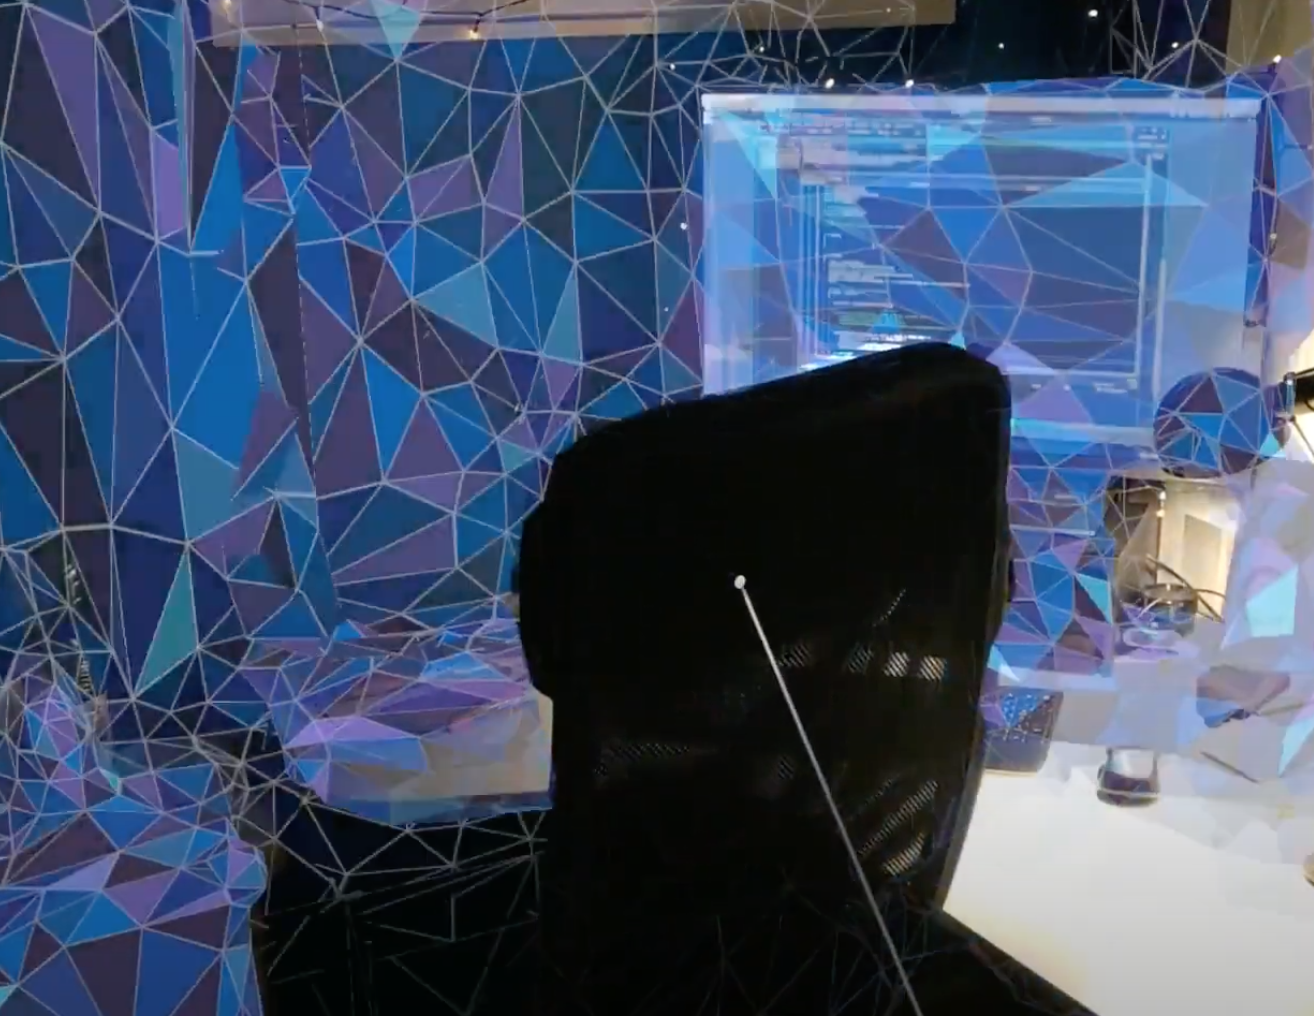
\includegraphics[width=0.47\textwidth]{gfx/hololens_env.png}
	\caption{\label{fig:holo2_env}HoloLens 2 maps itself with a mesh.}
\end{wrapfigure}

Nowadays different HMD with varying performance levels and prices are available on the market. In this thesis, Microsoft HoloLens 2 was used for MR experience and data collection. It is an updated version of the previous generation HoloLens 1 headset from Microsoft with such improved feature as display resolution, field of view, weight, battery lifetime. By using the AHAT (Articulated HAnd Tracking) depth camera, the HoloLens 2 can capture hand movements to obtain hand tracking data. The build-in tracking systems allows HoloLens to understand the environment around the user and to place stable and accurate holograms on the correct places where they intended to be by the developer of MR Application. The data used to track users is represented in the spatial map\footcite{https://docs.microsoft.com/en-us/hololens/hololens-environment-considerations}. When VR Application is starting on HoloLens, HoloLens uses unique environmental landmarks to locate itself in a space. The mesh graphic spreading over the space is seen, as illustrated in Fig. \ref{fig:holo2_env}, during the Application launch and this means a device is mapping to surroundings. As user moves with HMD on their head, built-in cameras continuously scan the environment and construct virtual world geometry for real-world objects. The primary stereo rendering component attached to HMD can be accessed from Unity and thus the position and orientation can obtained for thesis purposes. 

%##############################################
\section{Six degrees of freedom}
\label{sec:theorie:6dof} 
Term \textit{degrees of freedom} describes how users interact with a virtual environment and how they can move inside it. Within 3-DoF space user has only three possibilities: look left and right, look up and down and pivot left and right. 3-DoF space does not allow to move throughout the virtual space. Thus only rotational movement can be tracked. In 3-DoF VR Application multimedia content is the omnidirectional or spherical video, which represents an entire 360$^{\circ}$ environment on a virtual sphere \cite{6-dof_metrics}. In 3-DoF space HMD enables to display only a portion of the environment around a user. User is virtually positioned at the centre of a sphere as shown in Fig. \ref{fig:3and6dof}, media is displayed from an inward position and user can only change the viewing direction (i.e., by looking up/down or left/right or tilting the head side to side) \cite{6-dof_metrics} but can not interact with a media by moving closer/further. Wherever user moves with a HMD on their head, they will remain placed in the  at the centre of a sphere and distance to a content can not be changed.
\begin{wrapfigure}{R}{0.4\textwidth}
	\centering
	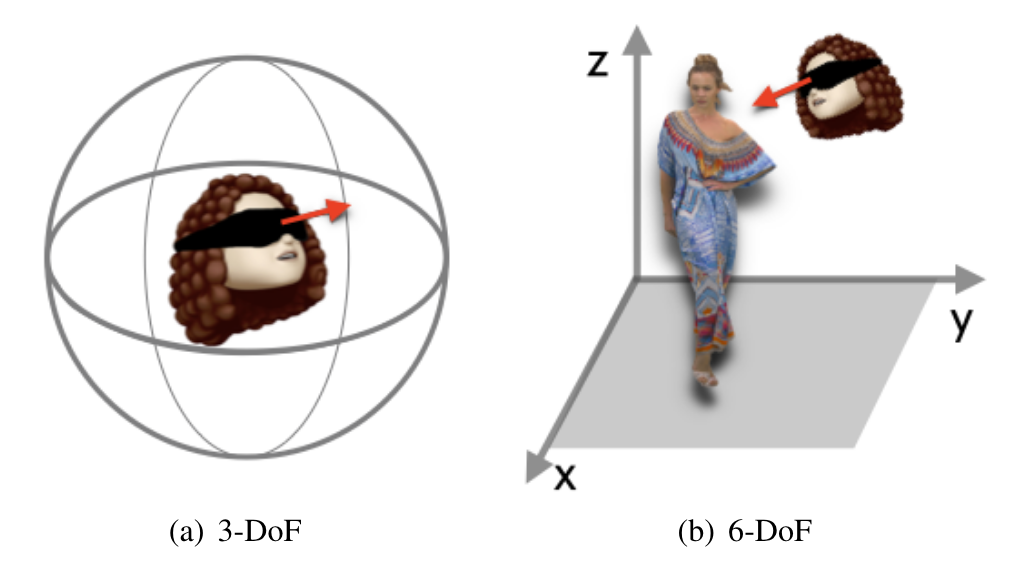
\includegraphics[width=0.37\textwidth]{gfx/3-6dof.png}
	\caption{\label{fig:3and6dof}Viewing paradigm in 3- and 6-DoF VR. Source: \cite{6-dof_metrics}}
\end{wrapfigure}

The new VR concept 6-DoF means tracking both position and rotation and refers to the freedom of movement of a rigid body in three-dimensional space. In 6-DoF VR Application user can also change viewing perspective by moving (e.g., walking, jumping) inside the virtual space \cite{6-dof_metrics}. Thus the scene is observed from an outward position in 6-DoF environment and extra degree of freedom transforms the virtual experience to be more natural and reflects to human movement in a three-dimensional space. Thus the VV and other volumetric objects such meshes or point clouds are used in MR Applications for 6-DoF scene population. User can freely walks inside the 6-DoF environment with a HMD on a head and observe the placed on scene volumetric objects from all points of view, and if the settings in Unity application allow physical interaction with objects, pick and move them on the new place. 

\section{Motion-to-photon latency}
\label{sec:theorie:m2p}
VR Application are deployed to the end-user with a goal to create an immersion of a physical presence in a non-physical world. In the real world there is no time delay between action taken and reaction observed. However, in AR/VR/MR Applications the difference between the user's head movement (action) and its corresponding display output reflections (reaction) is defined as motion-to-photon (M2P) latency. The presence of a delay between the physical movement and the display output worsens HMD user experience. In worst case even sense of physical presence in a virtual world would be lost. MTP latencies of more than 20 ms are experienced and cause spatial disorientation and dizziness, referred to as VR sickness or motion sickness \cite{delay_sickness, serhan_kalman}. Display lag can produce a range of other perceptual effects include degraded vision, compromised visuo-motor performance and motion sickness \cite{delay_sickness}. Different components of the HMD, such as the sensors, SOC, display and software can affect M2P latency. Reducing the M2P latency is the key to proving the best VR experience. Not only improving the device parameters, such a usage of more powerful HMD processor, need to be taken in account. VR Application developers must consider how to deploy more light-weighted applications. If the VR Application need to pull some data from the network or remote server, the network round-trip time and the added processing delays will increase the M2P latency compared to a system that only performs the processing locally \cite{serhan_kalman}.\\

\begin{wrapfigure}{L}{0.48\textwidth}
	\centering
	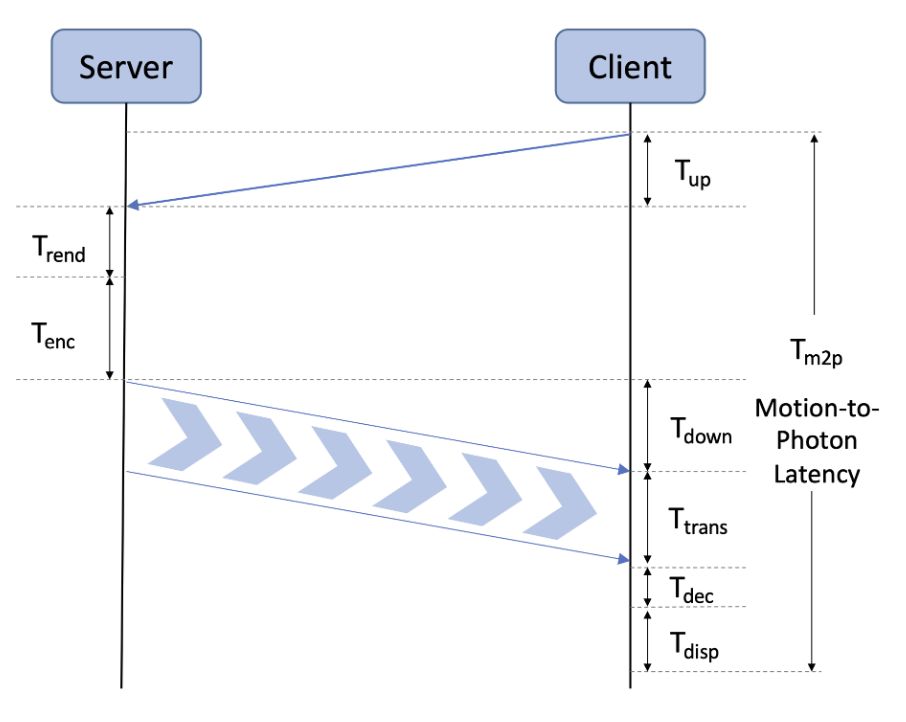
\includegraphics[width=0.46\textwidth]{gfx/m2p.png}
	\caption{\label{fig:m2p}M2P latency for a remote rendering system. Source: \cite{serhan_cloud_streaming}}
\end{wrapfigure}

As this thesis evaluates the reducing the M2P latency for VV streaming from remote cloud server, the Fig. \ref{fig:m2p} illustrates the different components of the M2P latency for a remote rendering system. Total M2P latency is equal to sum of the time taken by a bit of data to travel across the network from HMD to a server, server delay involved in computing the future user position and render a 2D view and a HMD delay during sensor measurements. If the user’s future head pose for a look-ahead time (LAT) equal to or larger than the M2P latency of the system could be predicted, it can eliminate M2P latency and improve the quality of the VR Applications. Studies showed that display lags of greater than 40 ms cause errors in tracking and following a target with the head \cite{delay_sickness}. This thesis evaluates the performance of RNN Models for LAT 100 ms that is higher than the measured M2P latency of a cloud-based volumetric streaming system described in the next section. 

\section{Cloud-based volumetric video streaming}
\label{sec:theorie:cloud}
% User Behaviour Analysis of Volumetric Video in Augmented Reality

\section{Challenges of head motion prediction}
\label{sec:theorie:head_pred}
All modern HMD has a position tracker, a device or a system of devices, that is responsible for reporting  the position and orientation of HMD to the computational unit that generates the virtual environment images displayed in the HMD. These images represent the view that a wearer of HMD would have seen if user was present in VR at the position and orientation reported by position tracker \cite{hmd}.\\
While the task of position tracking is performed by HMD hardware, the task of position prediction of the movement of human body in the virtual reality remains challenging, and it is still complicate to achieve high-precision estimation. Recurrent neural networks have recently shown promising results in many machine learning tasks, especially when input and/or output are of variable length and are coming as time series with a sequential order.  Unfortunately, the known problem of RNN that was observed many years ago by e.g., \textit{Bengio et al., 1994} that it is difficult to train RNNs to capture long-term dependencies because the gradients tend to either vanish (most of the time) or explode (rarely, but with severe effects) \cite{rnn_difficults}. New approaches are needed to be implemented to reduce the negative impacts of this issue. Since traditional recurrent unit overwrites its content at each time-step, a LSTM unit is able to decide whether to keep the existing memory via the introduced gates. The Long Short-Term Memory (LSTM) has a number of minor modifications \cite{empirical_evaluation} since it was initially proposed in work \cite{lstm_orig}. Another approach called a gated recurrent unit (GRU) can adaptively capture dependencies of different time scales without having a separate memory cells \cite{empirical_evaluation}. These two approaches can help to find the long-term dependencies in the data obtained from HMD that are otherwise are hidden by the effect of short-term dependencies from the standard RNN models.\\
%============================================
Not only the NN architecture is important for high prediction accuracy. Understanding how users interact and behave in AR or VR is a key for preparing the correct dataset when working with HMD's sensors. The experiment done by \textit{Zerman et al., 2021} found out that users preferred to stay in front of static point clouds and 1-1.5 meter away from them and spent more time looking at the frontal view and faces of human models \cite{user_behav_volumetric}. The navigation trajectories of users within a 6-Degrees-of-Freedom (DoF) should be additionally investigated. An extra level of interaction between user and content is available in 6-DoF environment. The user has now the freedom to change the viewing direction (rotating and translating the head as in 3DoF) but also to change position inside the VR environment \cite{new_challenge}. In a 3-DoF environment, users are viewing a portion of the omnidirectional content all the time being positioned at the centre of the spherical content. Thus it is important to understand that a distance between user and content is constant during the interaction \cite{new_challenge}. In a 6-DoF, however, the distance changes over time when user moves due to the added degrees of freedom. Thus viewport’s center position is not sufficient for tracking the trajectories, the additional metrics such the spatial coordinates and user orientation are needed to obtain the point of origin. Following \cite{new_challenge} \textit{Rossi et al, 2021} authored same year another work \cite{6-dof_metrics} dedicated 6-DoF metrics. Researchers proposed to change the video detailing based on user distance to the volumetric object. The closer users are to the volumetric content, the smaller and more detailed is the portion of the displayed content; the farther they are, the bigger but with fewer details becomes the displayed portion \cite{6-dof_metrics}. \textit{Rossi et al, 2021} experimented with different metrics to perform clustering in order to detect group of users with similar behavior in VR. The most promising metric seems to be based on the user position on the virtual floor. Metrics based only on viewport center and distance failed in detecting the group of users, which in the ground-truth case form their own cluster, as similar and divided them instead in different clusters \cite{6-dof_metrics}. For the trajectory detection best performed a metrics based on user position on the virtual floor, distance and viewport center. Thus not only the way in which users interact within a 3- and 6-DoF environment is fundamentally different. New physical settings and locomotion functionalities given to users also prevent a straightforward extension of current 3-DoF algorithms to 6-DoF \cite{6-dof_metrics}. The analysis above leads to the conclusions that prediction of the user's position and orientation on 6-DoF not only a contemporary but also a challenging task that requires new metrics and approaches to be investigated and implemented. 
% !TeX spellcheck = en
\chapter{Related work}
\label{sec:related}
This chapter presents the overview of previous research in the field of the prediction of user position. It includes both approaches for 3-DoF and 6-DoF environment, focusing on time series methods, Kalman Filter and overview of different  Recurrent Neural Network architectures such as LSTM and GRU.  


\section{Time series methods}
\label{sec:related:timeseries}

\section{Kalman Filter}
\label{sec:related:kalman}

KF-based extrapolation are deemed to be robust against fast fluctuations, but suffer from susceptibility to noise sensory data \cite{delay_compensation_360}.

\section{Recurrent Neuronal Network}
\label{sec:related:deep}
In this section the network architectures of most relevant works in the field head motion prediction with RNNs are explained and discussed whether LSTM or GRU architecture is better for the actual problem presented in this thesis. As was mentioned in section \ref{sec:related:timeseries}, typical HMD computes user positions in 6-DoF by using its tracker module and data comes as time series with a sequential order. The structure of an input is crucial and needed to be followed in order to predict the next future step for a look-ahead time correctly. A sequence of inputs can be processed with Artificial Neural Network (ANN) called Recurrent Neural Network (RNN). Moreover, RNN can processes input with remembering its state while processing the next sequence of inputs. In the last decade, RNN algorithms have been adopted for motion prediction of 3D sequences. For example, the work of \textit{Crivellari et al., 2020} targets traces of short-term tourists in a foreign country and tries to predict the motion of people in the environment they never seen before. LSTM-based model is used thus for analyzing the tourists’ mobility patterns \cite{tourist_traces}. The work of \textit{Yang et al., 2020} proposes using of flashbacks on hidden states in RNNs to search past hidden states with high predictive power. Authors mentioned that their approach gives an ability to determine a specific Point of Interests (POIs) from user’s mobility trace stored as a sequence of check-ins in Based Social Networks (LBSNs). Exploring the dataset researchers found sparsity and incompleteness of input sequences and thus the sequential pattern is difficult to be captured by RNNs. They considered temporal distances between similar POIs by flashing back to the historical hidden states sharing a similar temporal context as the current one \cite{rnn_traces_hidden}. \\
%================================================
The authors \textit{Aykut et al., 2018} claims their research to be first work that applies deep learning for head motion prediction. The current three rotations in three dimensions the so-called Euler angles as well as past values thereof within a certain time window (W) used as input for the network \cite{delay_compensation_360}. The best results delivered when 20 last values for each orientation direction (W = 250 ms) were used \cite{delay_compensation_360}. Instead of the absolute orientation values \textit{Aykut et al., 2018} suggest for a goal of generalization for other datasets to subdivide the inputs into their respective orientation groups and compute their normalized differences \cite{delay_compensation_360}. The authors experimentally confirmed that Feed-forward Neural Network (FFN) indeed had difficulties to learn for different delays even after an architecture was extended with the present delay and injected into all NN nodes. The using of LSTM-based architectures \textit{Aykut et al., 2018} reasoned with feedback loop and ability to establish a way of memory and share weights over time \cite{delay_compensation_360}. Researchers used Adam optimization algorithm, the maximum number of epochs was set to 1000, early stopping technique (patience = 2, min. delta = 0) was used to avoid overfitting. Additionally, the learning rate was decreased by 70\% from initial value of 0.001 every 30 epochs. The batch size B was set to $2^{11}$. Rectified Linear Unit (ReLU) as activation function for the FFN layers used with LSTM \cite{delay_compensation_360}. Three different architecture were tried. In all variants an input for NN was subdivided into dimensions and normalized within time window W set to 250 ms with $\triangle$t = 25 ms. Thus the length of input vector is equal to 10. Final result obtained from each NN variant is a vector of length of 10 for each pan, tilt and roll dimension separately containing future prediction with LAT 1s and step of 0.1s. \\
Conducted by researchers experiments showed that the LSTM-based architecture leads to a significant improvement of the MAE and RMSE metrics. The best performance is achieved by the interleaved architecture of LSTM and dense FFN blocks \cite{delay_compensation_360}. The LSTM-based methods were compared also to widely used approaches like the Linear Regression and a Kalman Filter based optimal state estimate. Thus \textit{Aykut et al., 2018} demonstrated a substantial improvement of the deep predictor for latencies in the range of 0.1–0.9 s \cite{delay_compensation_360}.\\ 
%================================================
Next year \textit{Aykut et al., 2019} experimented in their work \cite{telepresence} with GRU model that belongs to the group of recurrent neural networks (RNN). Authors mentioned that they already achieved best performance for headmotion prediction with LSTM as described before. However they tried an usage of dense GRUs combined with convolutional components regarding that fact that GRU is computationally more efficient, as it has fewer parameters and states than LSTM units \cite{telepresence}. The GRU-CNN-based network also receives pan, tilt, and roll present and past values within the same W = 250ms for last 20 values. Network trained on the normalized differences instead of using of the absolute values as it was done in \cite{delay_compensation_360}. A convolution layer performs as low-pass filter and reduces the noise. The core of the network consists of an interleaved structure of six dense GRUs each with 30 nodes and subsequent convolution units (kernel size 30x30), which compute the most distinct features. Max pooling layer down-samples the output of the last convolution layer and keeps the most significant features. The last step is passing the results through dense FFN and inverse remapping to the absolute orientation values. The model also predicts whole sequence of orientation values with LAT 1s and step of 0.1s as in \cite{telepresence}. The number of epoch in training remains the same as in \cite{delay_compensation_360} but early-stopping technique has higher patience parameter and equal 10. Compared to \cite{delay_compensation_360} the batch size was reduced to $2^{9}$. The rest of model parameters remains the same as in previous work of \textit{Aykut et al., 2018}. Authors said that proposed GRU-CNN-based network is able to improve the MAE and RMSE compared to all Kalman Filter and described above LSTM-CNN methods, especially for larger delays \cite{telepresence}. \\
%================================================
Researchers \textit{Karim et al., 2018} developed long short term memory fully convolutional network (LSTM-FCN). In the proposed models, the fully convolutional block is augmented by an LSTM block followed by dropout. The fully convolutional block consists of three stacked temporal convolutional blocks with filter sizes of 128, 256, and 128 respectively \cite{lstm_fcn}. Each convolutional block is identical to the convolution block in the CNN architecture proposed by \textit{Wang et al., 2018} in their work \cite{timeseries_scratch}. This means the basic block is a convolutional layer followed by a batch normalization layer and a ReLU activation layer. The convolution operation is fulfilled by three 1-D kernels with the sizes {8, 5, 3} without striding \cite{timeseries_scratch}. \textit{Wang et al., 2018} excluded in their FCN any pooling operation to prevent overfitting. Batch normalization helps to reduce generalization error. Global average pooling layer reduces the number of weights. Softmax layer produces the final labels \cite{timeseries_scratch}. The LSTM block, comprising of either a general LSTM layer or an Attention LSTM layer, is followed by a dropout. The output of the global pooling layer from FCN output and the LSTM block is concatenated and passed onto a softmax classification layer \cite{lstm_fcn}.\\
The important detail is that FCN block and LSTM block perceive the same time series input in two different views. If there is a time series of length N, the fully convolutional block will receive the data in N time steps \cite{lstm_fcn}. \textit{Karim et al., 2018} sends additionally the time series input into a dimension shuffle layer. Thus LSTM block receives transformed input having N variables with a single time step. Authors say that without the dimension shuffle, the performance of the LSTM block is significantly reduced due to the rapid overfitting of small short-sequence \cite{lstm_fcn}.\\
%================================================
In work of \textit{Chang et al., 2020} LSTM-based model is proposed to predict displacement of positions in each timestamp given measured acceleration and Euler angles from sensor signals \cite{6DoF_Tracking}. In addition to standard LSTM networks, they also use bidirectional LSTM (Bi-LSTM) networks, which is stacked two LSTM networks in forward and backward directions. Standard LSTM networks can only consider the past information and Bi-LSTM networks can capture both past and future information by two opposite temporal order in hidden layers \cite{6DoF_Tracking}. Authors predicted first displacement $x_{t_2} - x_{t_1}$ over the time interval $[t1, t2]$ and used it to obtain the position. Experimentally, authors found that the basic LSTM performs the best comparing to Bi-LSTM and Temporal Convolutional Network. Thus LSTM network with 3 layers used in this paper as the main structure.\\
%================================================
The paper \cite{action_recognition} also aims for action recognition using sensor signals from HMD. This approach presents another combination of of gated recurrent unit and additional model. Convolutional Auto-Encoder (CAE) model in a clustering fashion learns discriminative feature representation and helps to conquer difficulty of recognizing similar actions. As in the work \cite{6DoF_Tracking}, a deep sequential model learns the temporal representations and predicts the displacement of positions with acceleration and Euler angle to reduce error accumulation. Similar to \cite{6DoF_Tracking}, researches also used additionally a bidirectional LSTM (Bi-LSTM) network. The usage of CAE is proposed as a feature extraction model for feature representation of action signals and is composed of an encoder and decoder \cite{action_recognition}. The encoder contains two 2D convolutional layers with a kernel of size 3 × 1 with the stride of 1. The decoder contains two 2D transposed convolutional layers with the same kernel size and stride. The bottleneck is three feed-forward fully-connected layers with neurons of 1024, 128, and 1024, respectively. The tanh function is used as the activation function between the convolution layer and the fully connected layer \cite{action_recognition}. Input contains body acceleration, gravity acceleration, gyroscope, and quaternion with dimension equal to 26. The action signal is divided into segments of 25 timestamps by stride-1 sliding windows In this approach an action is performed and recorded separately and ground-truth labels was assigned. Then, the signals of each action with ground-truth labeling are used as input to CAE model for feature extraction by sliding windows \cite{action_recognition}. Authors mentioned a representation of a signal data by the latent vector in the low-dimensional space after using the CAE model. The latent vector then will be clustered by K-Means Clustering so that centroids are referred to as motion bases in a model. For action tracking with LSTM, the displacement in each timestamp was predicted first and then added to its previous location, instead of predicting each position directly \cite{action_recognition}. Similar as in work \cite{6DoF_Tracking} the 3-layered LSTM model performed better compared to Bi-LSTM. Authors said that the possible reason could be the short-term correlation of human actions in their dataset and that Bi-LSTM with its complicated model structure is rather suitable for long-term actions \cite{action_recognition}.\\
%================================================
The paper of \textit{Chung et al., 2014} should be noted separately in the end of related works review because it provides an interesting compassion and evaluation of the performance of recurrent units LSTM and GRU on sequence modeling. Authors mentioned the ability of LSTM to keep the existing memory via the introduced gates and thus to detect an important feature from an input sequence at early stage, to easily carry this information (the existence of the feature) over a long distance, hence, capturing potential long-distance dependencies \cite{empirical_evaluation}. The GRU takes linear sum between the existing state and the newly computed state similar to the LSTM but does not have any mechanism to control the degree to which its state is exposed, but exposes the whole state each time \cite{empirical_evaluation}. \textit{Chung et al., 2014} emphasize the fact that any important feature, decided by either the forget gate of the LSTM unit or the update gate of the GRU, will not be overwritten but be maintained as it is \cite{empirical_evaluation}. LSTM unit controls the amount of the new memory content and does not have any separate control of the amount of information flowing from the previous time step. The GRU differs and controls the information flow from the previous activation when computing the new and does not independently control the amount of the candidate activation being added via update gate \cite{empirical_evaluation}. The experiments provided in this work clearly indicate the advantages of the gating units over the more traditional recurrent units. \textit{Chung et al., 2014} mentioned that with dataset they used GRU unit outperformed LSTM unit. But they suggest that the choice of the type of gated recurrent unit may depend heavily on the dataset and corresponding task \cite{empirical_evaluation}. Thus in section \ref{sec:design:dataset:explor} of chapter ``Data and Model'' the data exploration of the obtained from HMD Microsoft HoloLend is done in order to understand the dataset before the beginning with a development of model architecture. 
% !TeX spellcheck = en
\chapter{Data and Model}
\label{sec:design}
This chapter presents the steps of development and implementation of the proposed approach. The Unity Application for HoloLens was deployed on HMD and a raw data with measures and dimension columns was obtained. This data than was analyzed and preprocessed to ensure that the captured data can be used in corresponding machine learning models. The model architecture was implemented and experimentally improved during training and evaluation steps. 

\section{6-DoF Dataset}
\label{sec:design:dataset}
This section describes how the dataset was obtained, analyzed and presents the visualization of user's head position and rotation. The real 6-DoF dataset must be used as training data from which the model can learn the spacial and time dependences. This step is crucial for a high accuracy prediction and almost all machine learning approaches requires not only row data collection but also data exploration and data preprocessing steps to be done before training begins.

\subsection{Data collection from HMD}
\label{sec:design:dataset:HL}
In this master thesis HoloLens 2, the second iteration of Microsoft's head-mounted mixed reality device, was used for data collection. The user position and orientation were obtained with Unity application developed for this purpose. Main Camera in Unity is automatically configured to track head movements. More details about Unity application can be found in section \ref{sec:imp:programming:unity}.\\
Using the Main Camera, a user position $(x, y, z)$ and orientation in quaternion $(qx, qy, qz, qw)$ were logged in a $csv$-file. Quaternions obtained from HMD will be used to define a rotation by four numbers. Quaternions representations are very convenient for operations such as composition or rotations and coordinate transformation \cite{principles_robot_motion_book}. For these reasons quaternions are chosen for the representation of user head's rotation in three dimensions. Comparing to dataset in \cite{serhan_kalman}, the additional parameters were recorded from the Main Camera in order to add more information during training processes. Thus the world-space speed of the camera in meters per second was recorded. Unity velocity has the speed in $(x, y, z)$ defining the direction. The obtained 6-DoF dataset has 10 features used in training process: position $(x, y, z)$, orientation  $(qx, qy, qz, qw)$ and velocity $(x, y, z)$.\\
The datasets were recorded in the laboratory space. HMD was presented to users and the basic functions were explained. During data recording, users freely walked wearing HMD in laboratory space. The Unity application, running on HMD, not only recorded the mentioned before parameters but also had a volumetric animated object placed placed 3 meters ahead of the user in the Mixed Reality environment. No personal data was recorded during these sessions and all traces are obtained anonymously. Thus, after an Unity application was launched, user could immediately see the animated object. The several traces were recorded at least for 10 minutes each. It allows to have enough data after splitting the dataset into training, test and validation partitions. Table \ref{tab:raw_data} show the first 20 rows from raw dataset obtained from HoloLens 2 and used in training. As mentioned above, 6-DoF dataset has 10 columns, thus the table \ref{tab:raw_data} presents only $timestamp$ and position $(x, y, z)$ columns. 

\begin{table}[!ht]
		\footnotesize
		\centering
	\begin{tabular}{|l|l|l|l|}
		\hline
		timestamp & x & y & z \\ [0.5ex] 
		\hline\hline
		2.649431 & 0.004954389 & 0.003402365 & 0.01010712 \\ \hline
		2.66943 & 0.00459053 & 0.003120769 & 0.01130438 \\ \hline
		2.698009 & 0.003960807 & 0.002990472 & 0.01276976 \\ \hline
		2.719285 & 0.003730714 & 0.003037783 & 0.01305151 \\ \hline
		2.746641 & 0.003252693 & 0.003489003 & 0.01368421 \\ \hline
		2.764094 & 0.003153284 & 0.003518121 & 0.01400959 \\ \hline
		2.780033 & 0.003087142 & 0.003409061 & 0.01435899 \\ \hline
		2.802086 & 0.003021815 & 0.00314023 & 0.01473305 \\ \hline
		2.815575 & 0.002789935 & 0.003551113 & 0.01506916 \\ \hline
		2.832602 & 0.002527435 & 0.003542757 & 0.01534094 \\ \hline
		2.848514 & 0.002212256 & 0.003605011 & 0.01565307 \\ \hline
		2.863769 & 0.001921757 & 0.003369405 & 0.01590317 \\ \hline
		2.879648 & 0.001668522 & 0.00348538 & 0.01607716 \\ \hline
		2.89686 & 0.001501704 & 0.003624826 & 0.01627397 \\ \hline
		2.913541 & 0.001487849 & 0.00359472 & 0.01643924 \\ \hline
		2.930006 & 0.001501501 & 0.003769569 & 0.01669565 \\ \hline
		2.948201 & 0.001617525 & 0.004252479 & 0.01697758 \\ \hline
		2.964302 & 0.001755987 & 0.004224311 & 0.01721937 \\ \hline
		2.97978 & 0.001838901 & 0.004487753 & 0.01747578 \\ \hline
		2.997117 & 0.002005509 & 0.005007531 & 0.01782864 \\ \hline
	\end{tabular}
\caption{\label{tab:raw_data}Raw data from HoloLens 2}
\end{table}

The first column in dataset is $timestamp$. It is obviously, that timestamp appears in row dataset not linearly and comes with different pauses. Even the high-cost HMD, like used in this research HoloLens 2, is sometimes unstable in frame rate during collecting data\footnote{https://docs.microsoft.com/en-us/windows/mixed-reality/develop/advanced-concepts/hologram-stability}.  In the Unity Application, the frame rate is  60 Hz which means that data will be collected per 0.016(6) second. Unfortunately, HMD could have delays, and the time gap of two samples may be reduced or increased, as we can observe on raw dataset. Data on some expected timestamps may be unavailable in HMS for recording. Those sequences with fewer timesteps may be considered to have missing values. To deal with above situation, the preprocessing steps must be done. They are described in a section \ref{sec:design:dataset:preprocessing} below. 

\subsection{Data preprocessing}
\label{sec:design:dataset:preprocessing}
As was mentioned in section \ref*{sec:design:dataset:HL}, the raw sensor data obtained from the HoloLens was unevenly sampled at 60 Hz and had different temporal distances between consecutive samples. \textit{Gül et al., 2020} obtained the similar raw dataset from same HMD and interpolated it to obtain temporally equidistant samples. Same as it was done in work \cite{serhan_kalman}, the position and velocity data were upsampled using linear interpolation and for quaternions SLEP was used. During preprocessing step Euler angles (yaw, pitch, roll) were calculated from quaternions and these parameters are used for visualization purposes. Although the interpolated $csv$-file contains additional Euler angles columns, only described in section \ref{sec:design:dataset:HL} parameters were used for training and prediction. The table \ref{tab:inter_data} lists first 20 rows for columns $timestamp$ and position $(x, y, z)$ from interpolated dataset. This interpolated dataset is created with linear interpolation and SLEP mathematical methods from raw dataset shown in table \ref{tab:raw_data}. 

\begin{table}[!ht]
	\footnotesize
	\centering
	\begin{tabular}{|l|l|l|l|}
		\hline
		timestamp & x & y & z \\ [0.5ex] 
		\hline\hline
		0.0 & 0.004954389 & 0.003402365 & 0.01010712 \\ \hline
		5000000.0 & 0.004833102666666667 & 0.0033084996666666667 & 0.010506206666666667 \\ \hline
		10000000.0 & 0.004711816333333333 & 0.0032146343333333332 & 0.010905293333333333 \\ \hline
		15000000.0 & 0.00459053 & 0.003120769 & 0.01130438 \\ \hline
		20000000.0 & 0.004485576166666666 & 0.003099052833333333 & 0.011548609999999999 \\ \hline
		25000000.0 & 0.004380622333333333 & 0.0030773366666666667 & 0.011792839999999999 \\ \hline
		30000000.0 & 0.0042756685 & 0.0030556205 & 0.01203707 \\ \hline
		35000000.0 & 0.004170714666666667 & 0.003033904333333333 & 0.0122813 \\ \hline
		40000000.0 & 0.004065760833333334 & 0.003012188166666667 & 0.01252553 \\ \hline
		45000000.0 & 0.003960807 & 0.002990472 & 0.01276976 \\ \hline
		50000000.0 & 0.00390328375 & 0.00300229975 & 0.0128401975 \\ \hline
		55000000.0 & 0.0038457605 & 0.0030141275 & 0.012910635 \\ \hline
		60000000.0 & 0.00378823725 & 0.00302595525 & 0.0129810725 \\ \hline
		65000000.0 & 0.003730714 & 0.003037783 & 0.01305151 \\ \hline
		70000000.0 & 0.0036510438333333334 & 0.0031129863333333335 & 0.01315696 \\ \hline
		75000000.0 & 0.003571373666666667 & 0.003188189666666667 & 0.01326241 \\ \hline
		80000000.0 & 0.0034917035000000003 & 0.003263393 & 0.01336786 \\ \hline
		85000000.0 & 0.0034120333333333332 & 0.0033385963333333333 & 0.01347331 \\ \hline
		90000000.0 & 0.0033323631666666667 & 0.0034137996666666667 & 0.01357876 \\ \hline
		95000000.0 & 0.003252693 & 0.003489003 & 0.01368421 \\ \hline
	\end{tabular}
	\caption{\label{tab:inter_data}Interpolated data from HoloLens 2}
\end{table}


After the interpolated dataset was plotted as figure \ref{fig:inter_data}, the important observations based on the sample trace could be done. While the user position data plots look appropriate for machine learning algorithms, the two graphs with orientation show data that is not the perfect case for usage with machine learning technologies and could decrease the prediction rate. The real part $qw$ and the component $qy$ of quaternion and $yaw$ of Euler angles are obviously discontinuous making it hard for a predictor to learn. A orientation on quaternions is used in training, thus this data requires a few additionally preprocessing steps. Usually, when doing calculation with quaternions, quaternions must be normalized to a unit length in order to represent valid rotations \cite{principles_robot_motion_book}. The normalized quaternion can be calculated using formula:
\begin{equation}
U_g = \frac{q}{|| q ||} = \frac{w}{|| q ||} + i \cdot \frac{x}{|| q ||} + j \cdot \frac{y}{|| q ||} + k \cdot \frac{z}{|| q ||}
\end{equation}

where $|| q || $ is a magnitude and can be found with formula:
\begin{equation}
|| q || = \sqrt{w^2 + x^2 + y^2 + z^2 }
\end{equation}

During experiments with quaternions in dataset obtained from HoloLens was found that quaternion magnitudes $|| q ||$ in HoloLens dataset are equal to 1. Thus data came from HMD already normalized, so that a quaternion in dataset kept the same orientation as it was during user's movement but its magnitude is 1.0.


\begin{figure}[htb]
	\begin{center}
		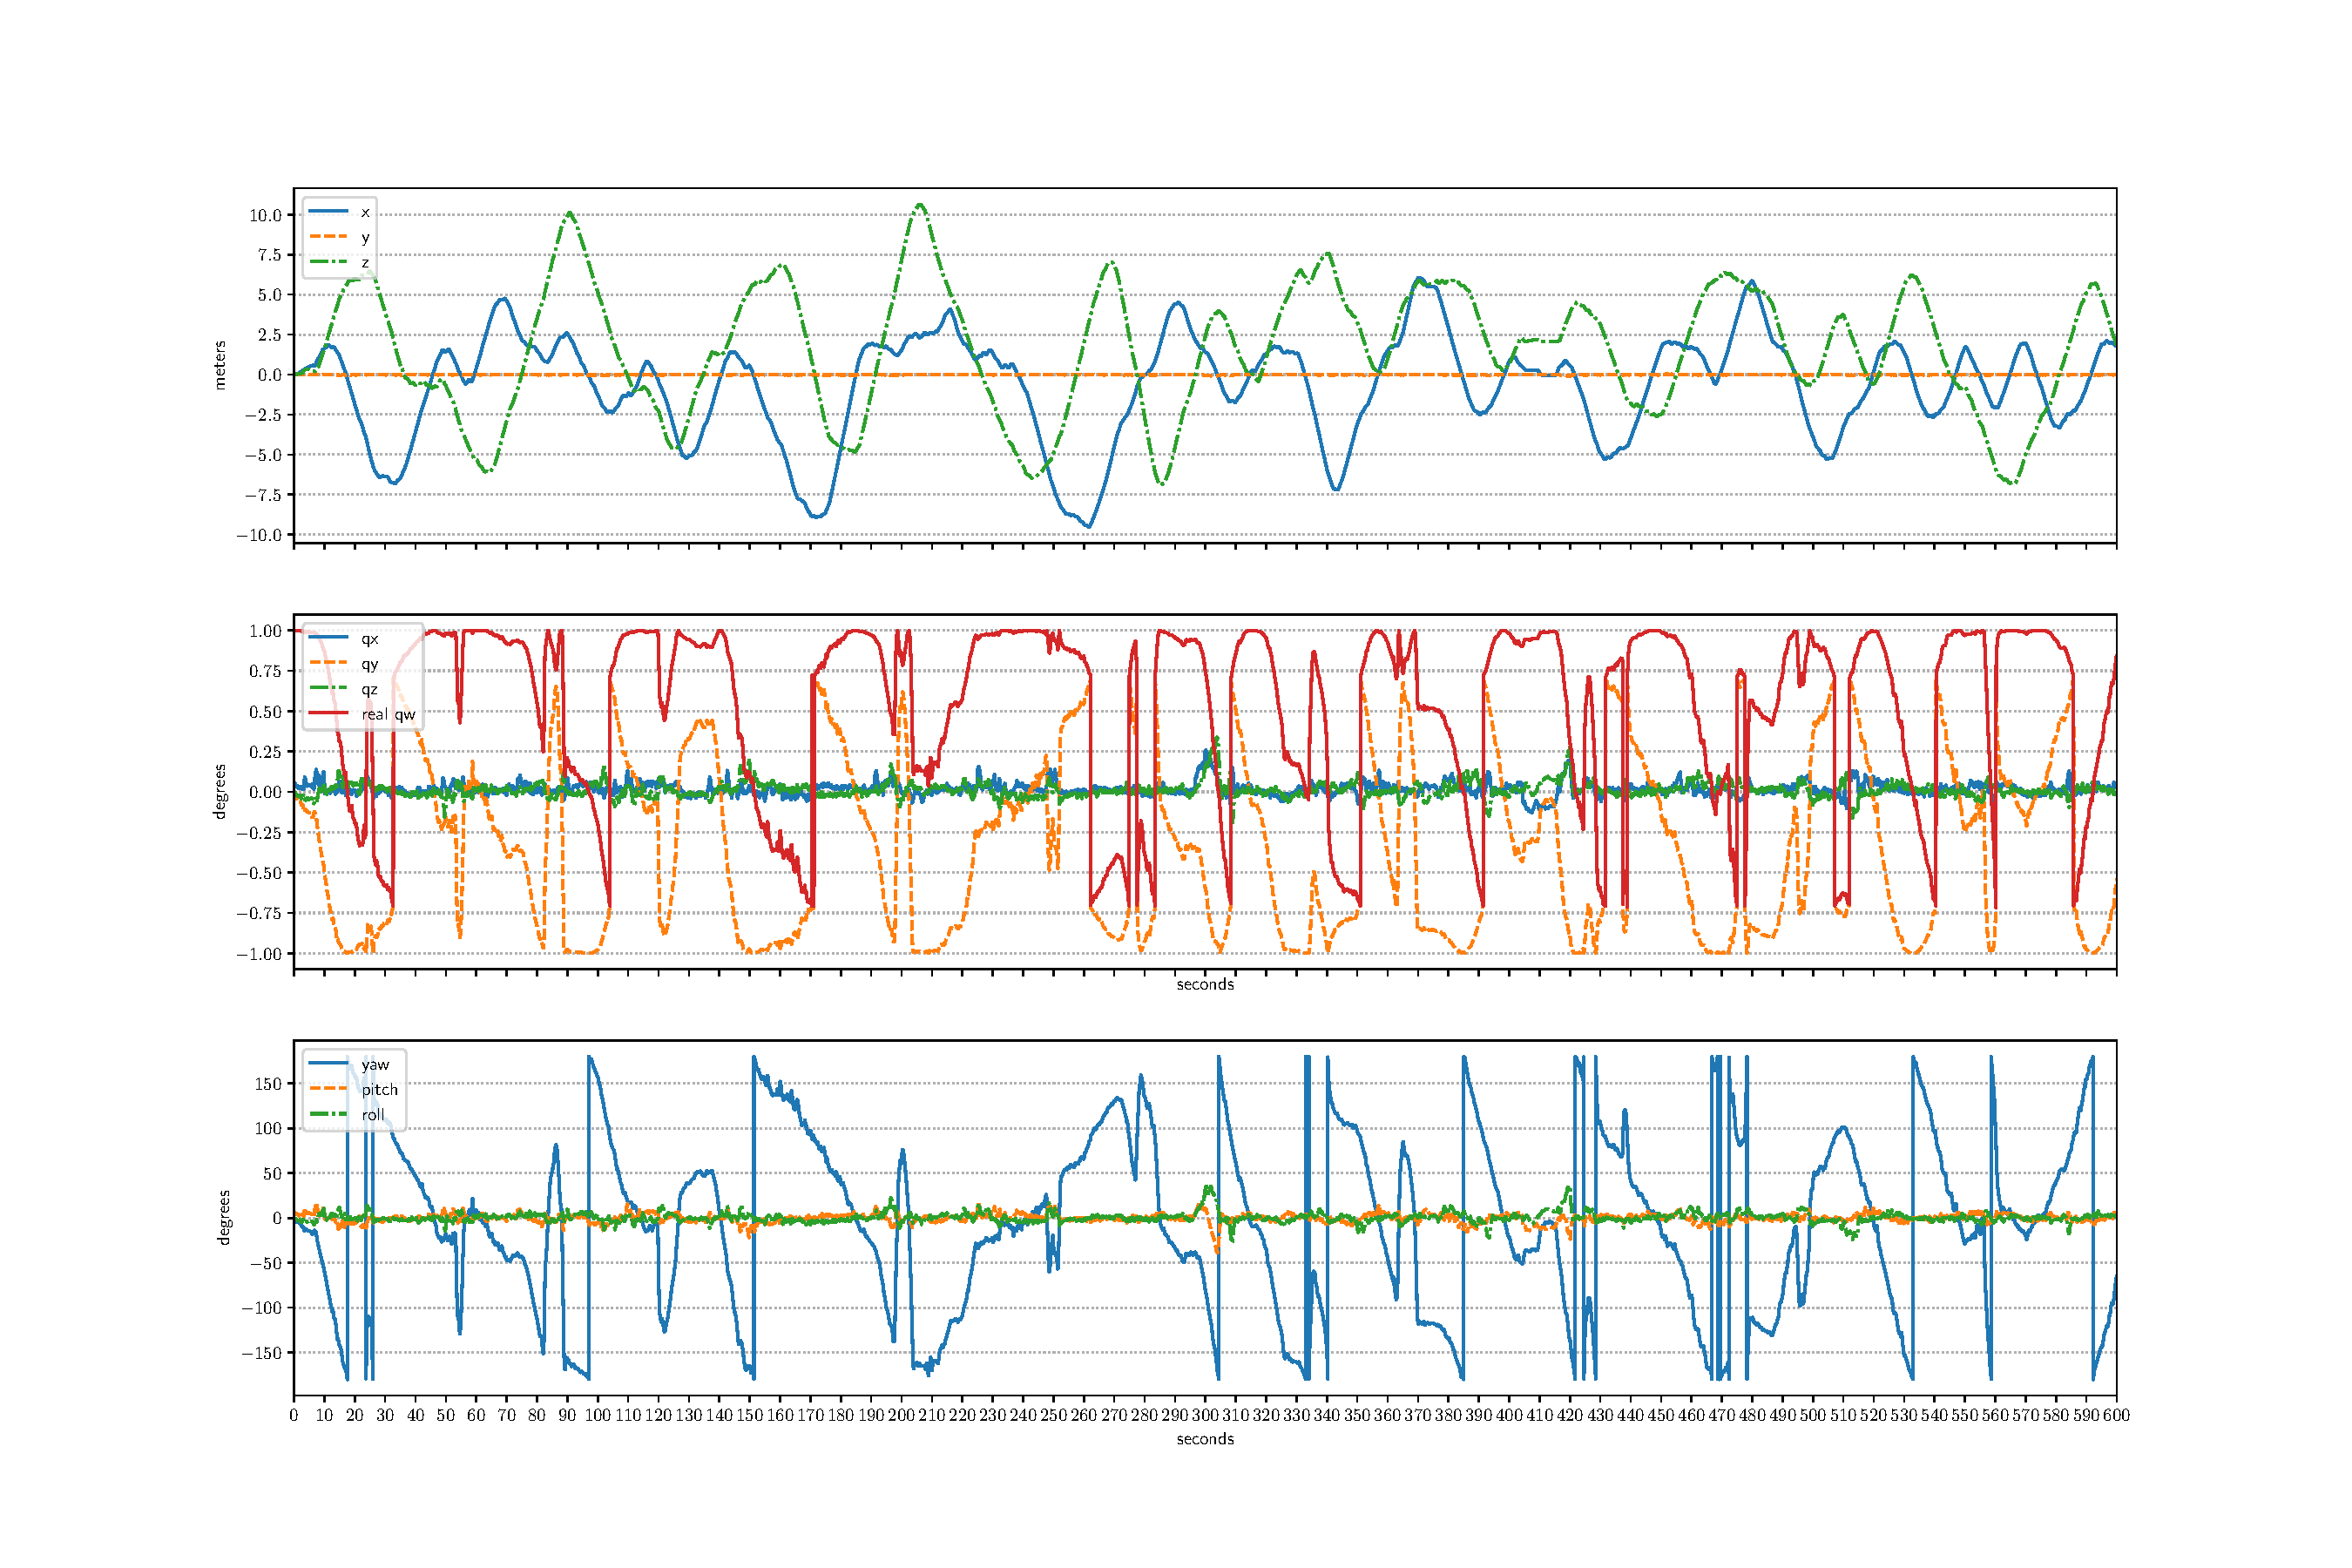
\includegraphics[width=1\textwidth, keepaspectratio]{gfx/Fig-1556-interpolated.pdf}
		\caption{\label{fig:inter_data}Interpolated 6-DoF dataset's user position and orientation in quaternions and Euler angles.}
	\end{center}
\end{figure}

Next, quaternions between neighboring points in obtained dataset represent the very similar orientation made by user wearing HMD step by step. The middle plot on figure \ref{fig:norm_data} has discontinuities that can be seen on $qw$ line. But regardless the discontinuity (sharp change of line from negative to positive area with the same amplitude) the two neighboring quaternions with similar rotation have significant 4D vector space between them. It makes prediction worse what can be proved by RMSE and MSE rotation metrics. Flipping the sign will not affect the rotation, but it will ensure that there are no large jumps in 4D vector space when the rotation difference in rotation space (SO(3)) is small. If negative component of quaternions will be flipped into positive then the dataset representing same rotation without creating an artificial discontinuity in the space will be available for model training. Thus after normalization step, the two representations of quaternions are blended into one data set, omitting to discontinuities in the time series as can be seen presented on Figure \ref{fig:norm_data}. Indeed, the RMSE and MSE rotation metrics were improved when model was trained with dataset with quaternions without sharp sign changes. More information can be found in sections \ref{sec:imp:experiments} and \ref{sec:imp:results}.

\begin{figure}[htb]
	\begin{center}
		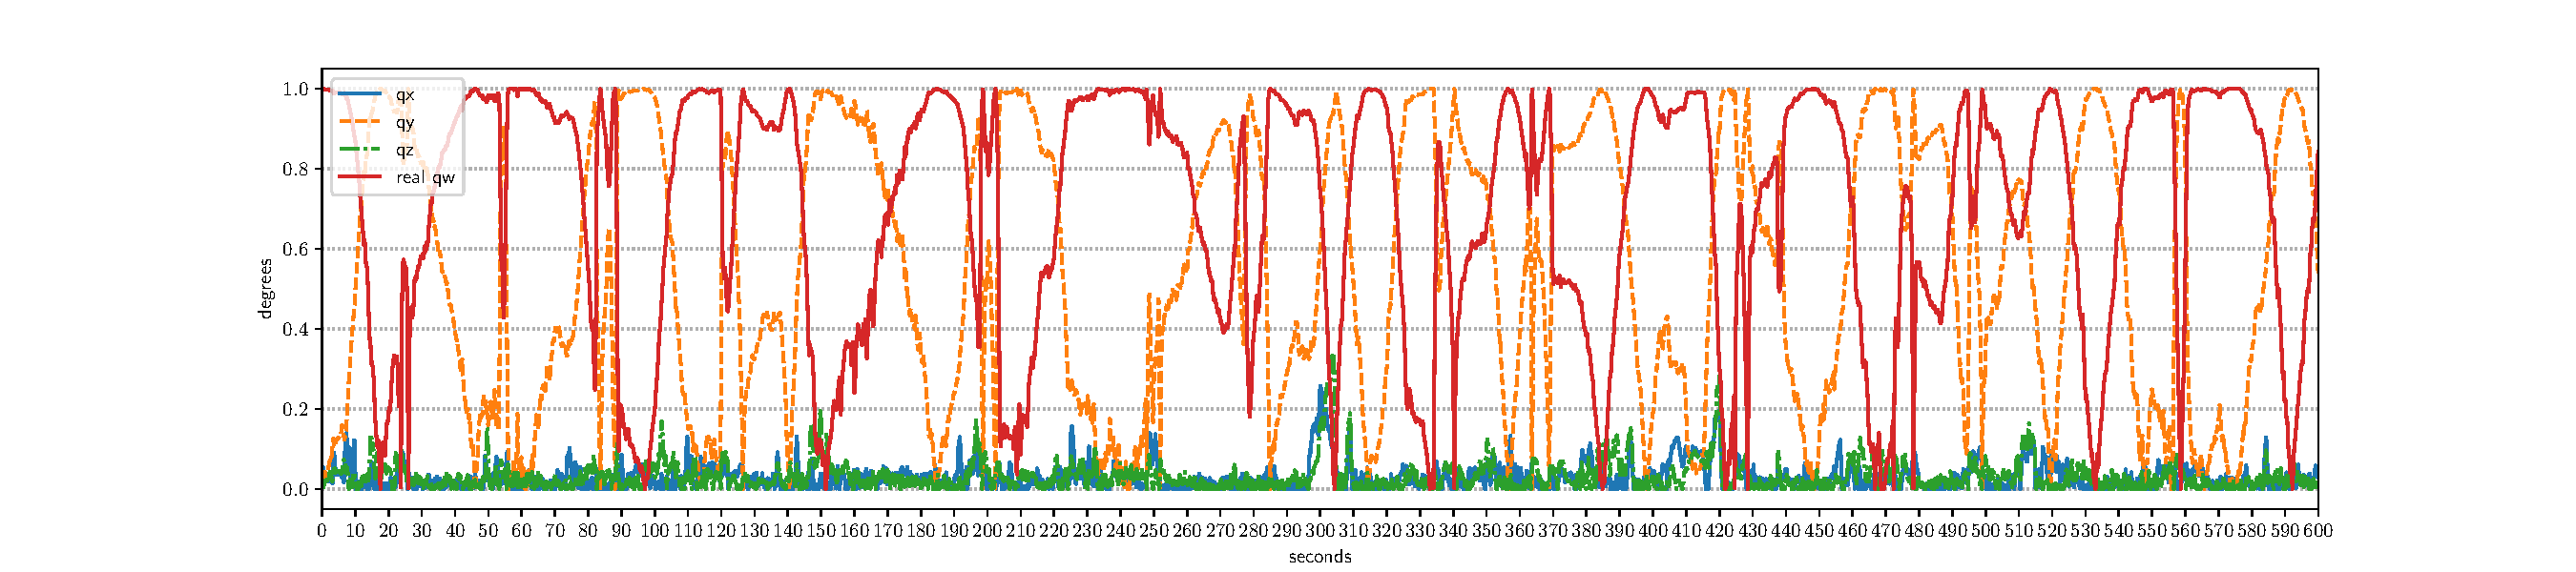
\includegraphics[width=1\textwidth, keepaspectratio]{gfx/Fig-1556-quaternions_flipped.pdf}
		\caption{\label{fig:norm_data} Quaternions from 6-DoF dataset's flipped if their real part is negative}
	\end{center}
\end{figure}

The figure \ref{fig:compare} represents quaternions of the original interpolated dataset on the upper part of the plot and the normalized flipped quaternions on the lower part of the plot. The quaternion's components were flipped only if the if their real part became negative. Different to figure \ref{fig:norm_data} the limit of y-axis is set to [-1, 1] on figure  \ref{fig:compare} so that the result of inverting of quaternion is easy co compare to original data.  Figure \ref{fig:norm_data} shows plotted data with length of 20 seconds in range 162 - 182 s from both datasets.

\begin{figure}[htb]
	\begin{center}
		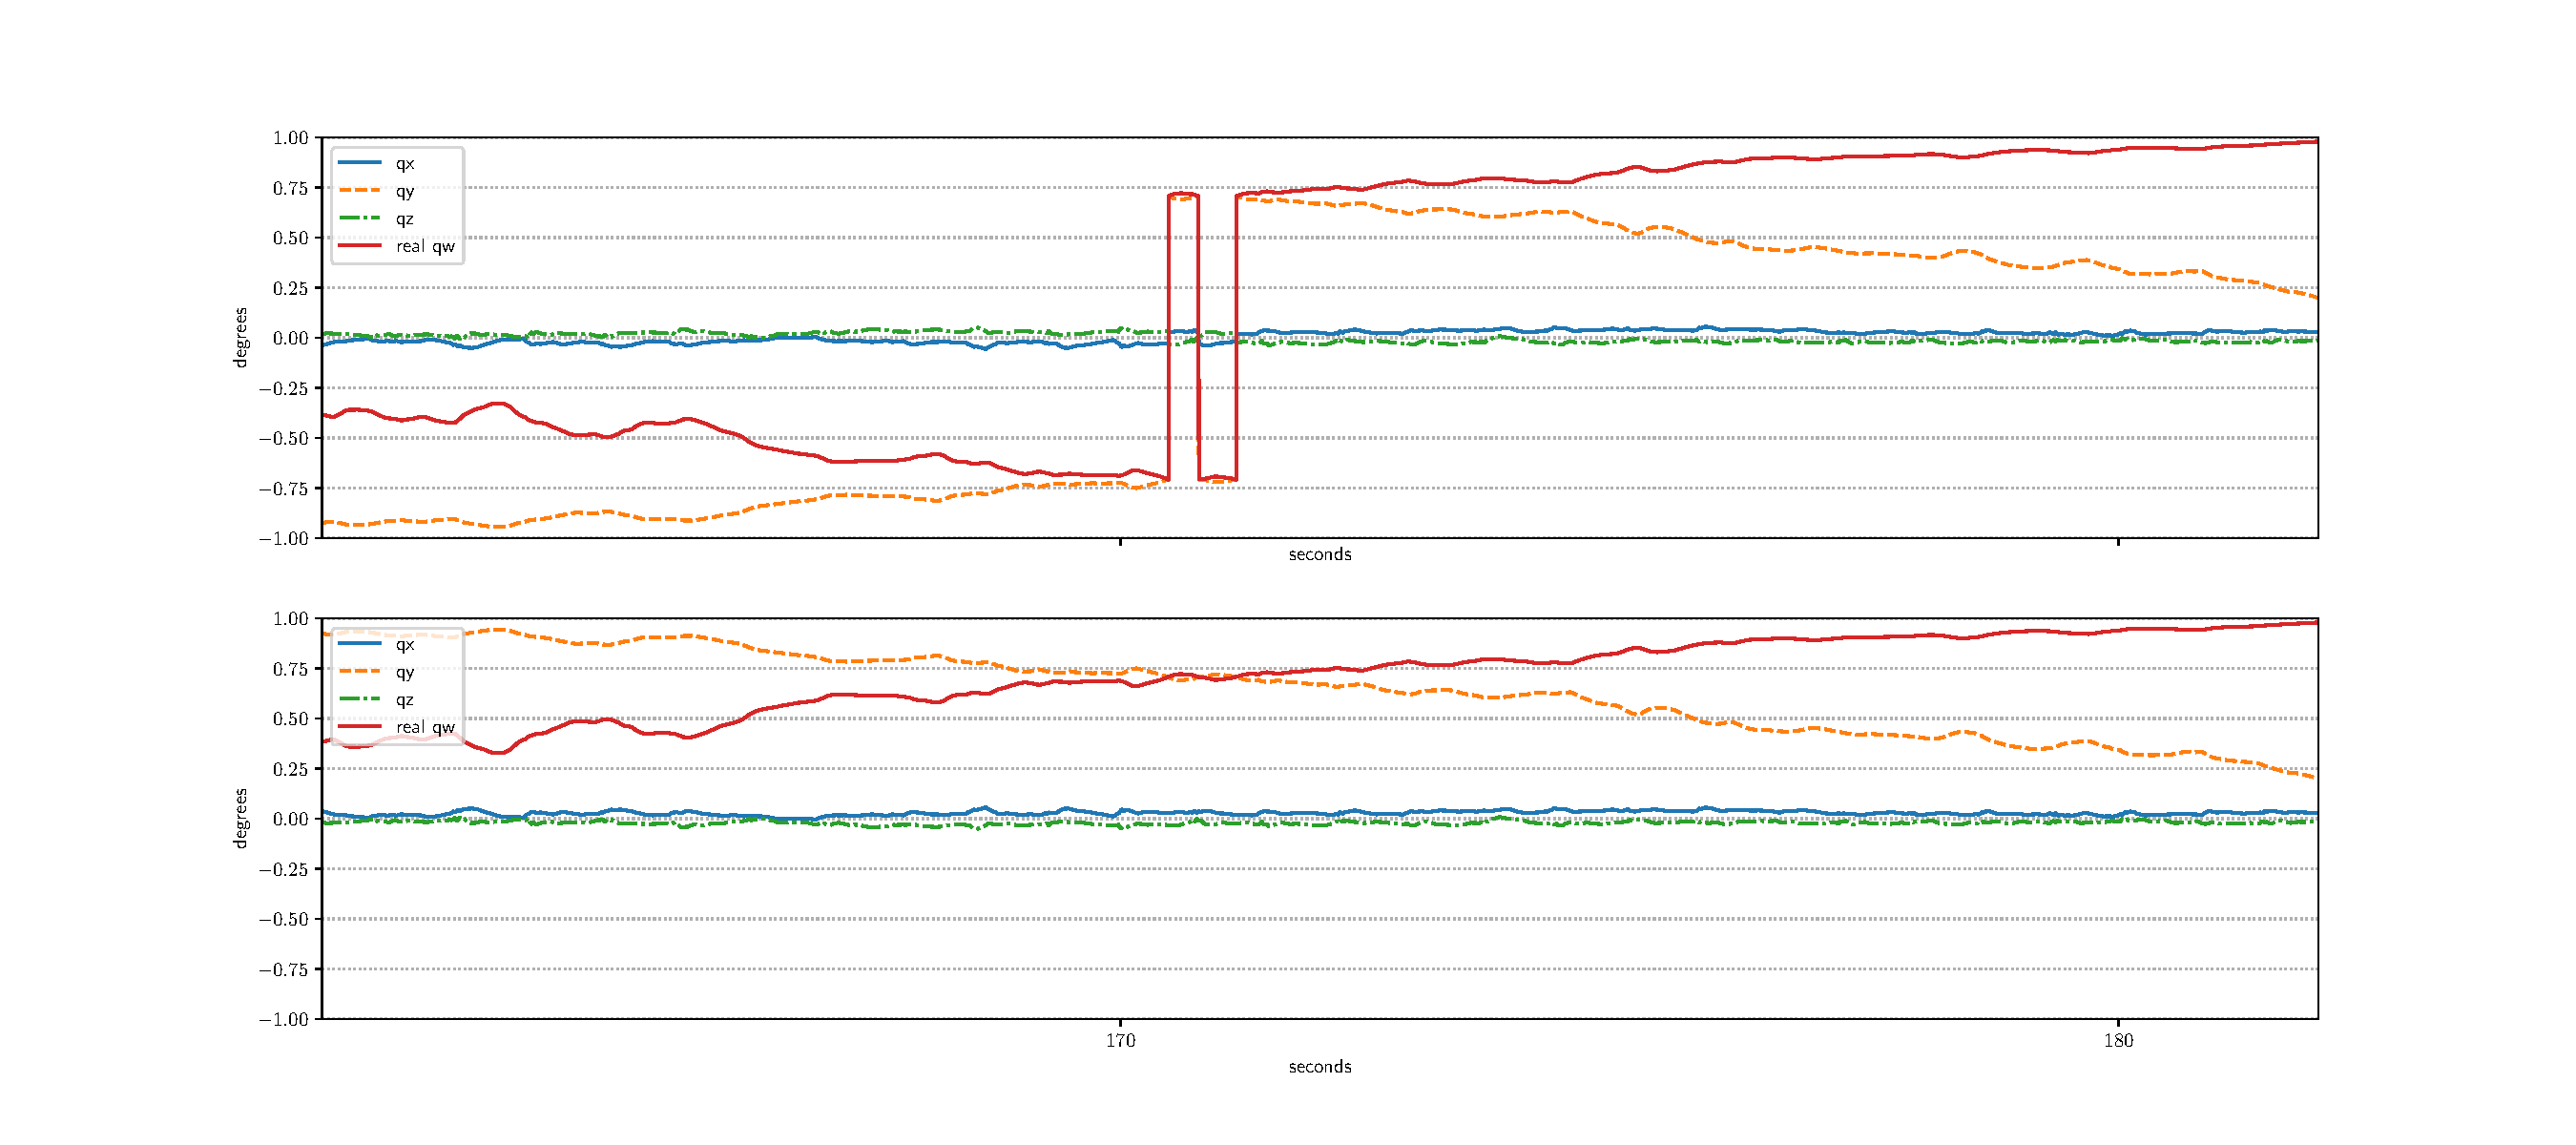
\includegraphics[width=1\textwidth, keepaspectratio]{gfx/Fig-1556-compare.pdf}
		\caption{\label{fig:compare} Quaternions from 6-DoF dataset's flipped if their real part is negative}
	\end{center}
\end{figure}



\subsection{Data Exploration}
\label{sec:design:dataset:explor}


!! Data analysis AVG linear velocity position, plots 

We can make two important observations based on the sample trace: firstly, the viewer rarely moves along the y-axis (except for the time period between 38-42 s during which the viewer probably sat down and stood back up), which is understandable since it requires more effort to crouch down and stand up. Secondly, the orientation changes are typically due to yaw movements, whereas the magnitude of changes due to roll and pitch movements are much smaller. Our observations are also confirmed by visual inspection of the other recorded traces.


\section{Neural Network}
\label{sec:design:nn}

\subsection{Network architecture}
\label{sec:design:nn:architecture}

\subsection{Network input}
\label{sec:design:nn:input}


\section{Training methods}
\label{sec:design:train}

% !TeX spellcheck = en






\section{Evaluation metrics}
\label{sec:imp:eval}


\section{Experiments}
\label{sec:imp:experiments}

\subsection{Datasets}
\label{sec:imp:experiments:ds}
As already stated in section \ref{sec:design:dataset:preprocessing}



\section{Results}
\label{sec:imp:results}

% !TeX spellcheck = en
\chapter{Analysis}
\label{sec:analysis}

The introduction text to analysis chapter

\section{Limitations}
\label{sec:analysis:limitations}

\section{Conclusion}
\label{sec:analysis:conclusion}

\section{Suggestions for future work}
\label{sec:analysis:future}


% !TeX spellcheck = en_EN
%\appendix
\clearpage
\pagenumbering{Roman}
\chapter*{Glossary}
\addcontentsline{toc}{chapter}{\protect\numberline{Glossary}}%
\section*{AJAX}
\label{sec:appendix:ajax}
AJAX (asynchrones Javascript und XML) ist der allgemeine Name für Technologien, mit denen asynchrone Anforderungen (ohne erneutes Laden von Seiten) an den Server gestellt und Daten ausgetauscht werden können. Da die Client- und Serverteile der Webanwendung in verschiedenen Programmiersprachen geschrieben sind, müssen zum Austausch von Informationen die Datenstrukturen (z. B. Listen und Wörterbücher), in denen sie gespeichert sind, in das JSON-Format konvertiert werden.


 
\pagenumbering{Roman}
\setcounter{page}{1}

\cleardoublepage


%\listoffigures
%\cleardoublepage
%\listoftables
%\cleardoublepage

% **************************************************
% End of Document CONTENT
% **************************************************

\printbibliography
\addcontentsline{toc}{chapter}{Bibliography}
%\lstlistoflistings

\end{document}
